% -------------------------------------------------------
%  Section 3: Proposed method
% -------------------------------------------------------
\section{روش پیشنهادی مقاله}
\label{sec:method}

\subsection{خط لوله}
محتوای دودویی فایل به‌صورت دنباله‌ای از بایت‌های بدون علامت خوانده و هر بایت یک پیکسل خاکستری تلقی می‌شود؛ دنباله با عرضی مشخص به ماتریس دوبعدی تا می‌خورد، محدوده بایتی هر بخش به یک زیرتصویر نگاشته می‌شود و همه زیرتصویر‌ها پس از تغییر مقیاس به $224 \times 224$ به‌عنوان کانال‌های یک تانسور ورودی روی هم می‌نشینند. مقاله به‌درستی تأکید می‌کند که نوع یک بخش را نمی‌توان از نام آن نتیجه گرفت (چون نام قابل مبهم‌سازی است) و ترکیب نام و صفات\pn{Characteristics} مبنا قرار می‌گیرد؛ برای \lr{BIG 2015} بخش‌ها به شش رده \lr{HEADER}، \kd{.text}، \kd{.rdata}، \kd{.data}، \kd{.rsrc} و «سایر» تقسیم می‌شوند.

\subsection{دو راهبرد قطعه‌بندی و پنج طرح داده}
تفاوت دو راهبرد در آن است که با فضای بیرون بخش هدف چه می‌کنند (شکل \ref{fig:splitmask}). در \textbf{\lr{Split}} پیکسل‌های هر بخش بیرون کشیده و فشرده بازچیده می‌شوند؛ چیدمان فضایی بخش نسبت به کل فایل به‌کلی دور ریخته می‌شود و ادعای مقاومت در برابر بازآرایی بخش‌ها دقیقاً از همین‌جا برمی‌خیزد. در \textbf{\lr{Mask}} زیرتصویر هم‌اندازه تصویر اصلی می‌ماند و تنها پیکسل‌های بخش هدف نمایش داده می‌شوند؛ اطلاعات مکانی حفظ می‌شود ولی به بهای تُنُکی شدید، که مقاله خود آن را علت افت \lr{S5} در حالت مستقل می‌داند.

\begin{figure}[!ht]
    \centering
    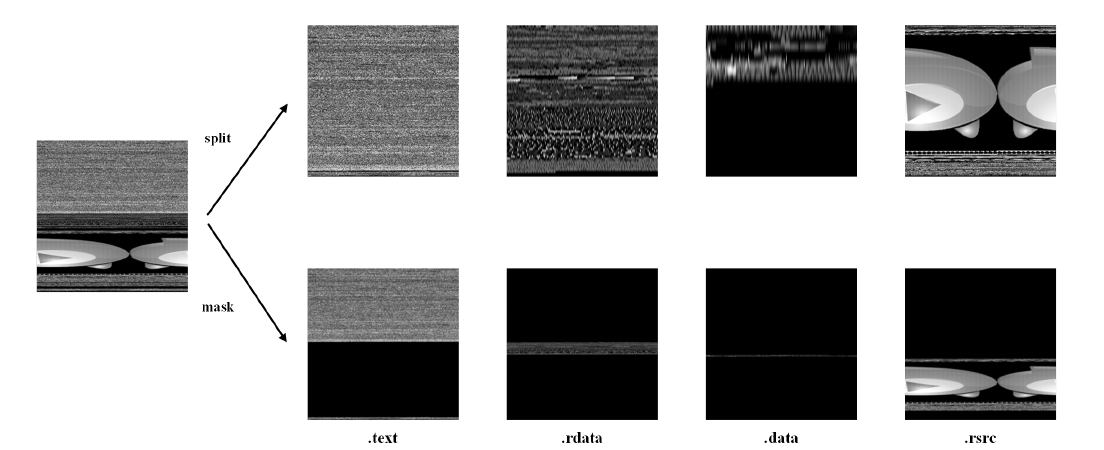
\includegraphics[width=0.78\textwidth]{figs/paper_splitmask.png}
    \caption{دو راهبرد قطعه‌بندی از شکل ۳ مقاله: \lr{Split} (ردیف بالا) هر بخش را فشرده و مستقل از جایگاهش بازمی‌چیند و \lr{Mask} (ردیف پایین) موقعیت اصلی را نگه می‌دارد و بقیه بوم را صفر می‌کند.}
    \label{fig:splitmask}
\end{figure}

بر این پایه پنج طرح داده تعریف می‌شود. سه طرح نخست به هم‌ترازی عرض مربوط‌اند: \lr{S1} عرض را از جدول اندازه‌فایل \lr{Nataraj} \cite{nataraj2011images} می‌گیرد (\num{۳۲} برای فایل‌های زیر \num{۱۰} کیلوبایت تا \num{۱۰۲۴} برای بزرگ‌تر از یک مگابایت)، \lr{S2} عرض را ریشه دوم اندازه فایل می‌گذارد و بیشترین تنوع عرض را می‌سازد، و \lr{S3} عرض را برای همه روی \num{۱۰۲۴} ثابت می‌کند. \lr{S4} و \lr{S5} همان \lr{Split} و \lr{Mask}اند و هر دو روی عرض ثابت \num{۱۰۲۴} بنا می‌شوند. در \lr{S1} تا \lr{S3} تصویر تک‌کاناله سه بار تکرار می‌شود تا با ورودی شبکه‌های از پیش‌آموخته سازگار شود؛ در \lr{S4} و \lr{S5} هر زیرتصویر یک کانال مستقل است.

\subsection{معماری‌ها}
مقاله از \lr{VGG16} \cite{simonyan2015vgg} و \lr{ResNet50} \cite{he2016resnet} از پیش‌آموخته روی \lr{ImageNet} استفاده می‌کند و برای پیکربندی‌های بیش از سه کانال، لایه پیچشی ورودی را بازتعریف می‌کند. مقاله در بخش محدودیت‌ها می‌پذیرد که این کار انتقال وزن‌های لایه نخست را مختل می‌سازد، اما چنان‌که در \S\ref{sec:critique} خواهیم دید، پیامد آن را در تفسیر جدول نتایج لحاظ نمی‌کند.
